\documentclass[12pt]{article}

%Import packages
\usepackage{amsmath}
\usepackage{listings}
\usepackage[utf8]{inputenc}
\usepackage{algpseudocode}
\usepackage{algorithm}
\usepackage[]{hyperref}
\usepackage{url}
\usepackage{pgfgantt}
\usepackage{comment}
\usepackage{array}
\usepackage[section]{placeins}
\usepackage{array,xstring}
\usepackage{numprint} 
\usepackage{pdflscape} %%landscape
\usepackage{rotating}
\usepackage{graphicx}
\usepackage{csvsimple}
\usepackage{siunitx}
\usepackage[top=2in, bottom=1.5in, left=1in, right=1in]{geometry}


%%config indice, referencias, metadata.
\hypersetup{
    pdftitle={Obligatorio 2 Middleware},
    bookmarksnumbered=true,     
    bookmarksopen=true,         
    bookmarksopenlevel=1,       
    colorlinks=true,            
    pdfstartview=Fit,           
    pdfpagemode=UseOutlines,
    pdfpagelayout=TwoPageRight,
    urlcolor=blue,
    linkcolor=blue,
    citecolor=red
}

% titulo
\title{Obligatorio 2 \\ Int. Middleware \\ Grupo 1 } 

% autores
\author{
  Cristiano Coelho 4.298.259-3\\
  Federico García 4.561.325-8\\
  Emiliano Conti 5.033.483-5\\
  Leonardo Clavijo 5.054.830-5
}

\date{\today}


\begin{document}
\maketitle

\begin{abstract}
En el presente documento se procede a la descripción de la arquitectura, el sistema de versionado,  y se define el modelo de calidad que permite medir el tiempo de respuesta de la aplicación.
\end{abstract}

\newpage
\tableofcontents
\newpage

\section{Introducción}
Dadas las características de un sistema que requiera la utilización de WebServices, el mismo puede encontrarse en constante evolución, por lo tanto se debe brindar un mecanismo de versionado que permita la interacción entre diversos sistemas, esto involucra sistemas legados, entonces es necesario mantener en funcionamiento la lógica del WebService anterior. Sin embargo dependiendo de las necesidades y la evolución del mismo servicio, puede ser necesario generar una nueva versión de los servicios web, pero al mismo tiempo todos los sistemas legados que utilizan este servicio deben poder realizar las operaciones aunque difiera del sistema nuevo.
Una forma de lograr mantener diferentes esquemas de negociación es a través del versionado, de esta forma se logra mantener el conjunto de sistemas legados y brindar un nuevo modelo para los sistemas recientes que requieran del nuevo servicio. Esto se puede lograr de diversas formas, manteniendo el servicio web activo o como en el caso del presente obligatorio, implementando un Proxy encargado de recibir las consultas de todos las versiones del servicio existentes, a partir de esto procesar las solicitudes dependiendo de la versión en la cual la solicitud es realizada. Para ello se describirá la arquitectura seleccionada, posteriormente el sistema de versionado, así como el modelo de calidad relativo al tiempo de respuesta tanto del servicio web como del Middleware implementado.

\section{Tecnologías}
Para la elaboración de el laboratorio se utilizaron las siguientes tecnologías y recursos, los Webservices se ejecutan en JBoss Application Server, a diferencia del primer obligatorio en el cual el Webservice se ejecutaba en un servidor Apache Tomcat. Esto se debe a las anotaciones y las tecnologías como ser MTOM, WS-Addressing y los tags de documentación para el versionado de los mismos.
\begin{itemize}
  \item JAX-WS
  \item JAX-RS
  \item Mule ESB
  \item SOAP UI
  \item JBoss Application Server 7
  \item MySQL
  \item Maven
\end{itemize}

\section{Arquitectura}
Se presenta el contexto y una breve descripción del mismo, para ello ver la figura \ref{fig:arq}.
Tenemos los siguientes entidades en el contexto:
\begin{itemize}
  \item Clientes Legacy: Los mismos utilizan el servicio en una versión no compatible.
  \item Clientes Nuevos: Utilizan la versión actual del servicio web.
  \item ESB: Middleware.
  \item Web Service SOAP.
\end{itemize}


  \begin{figure}[!h]
  \centering
    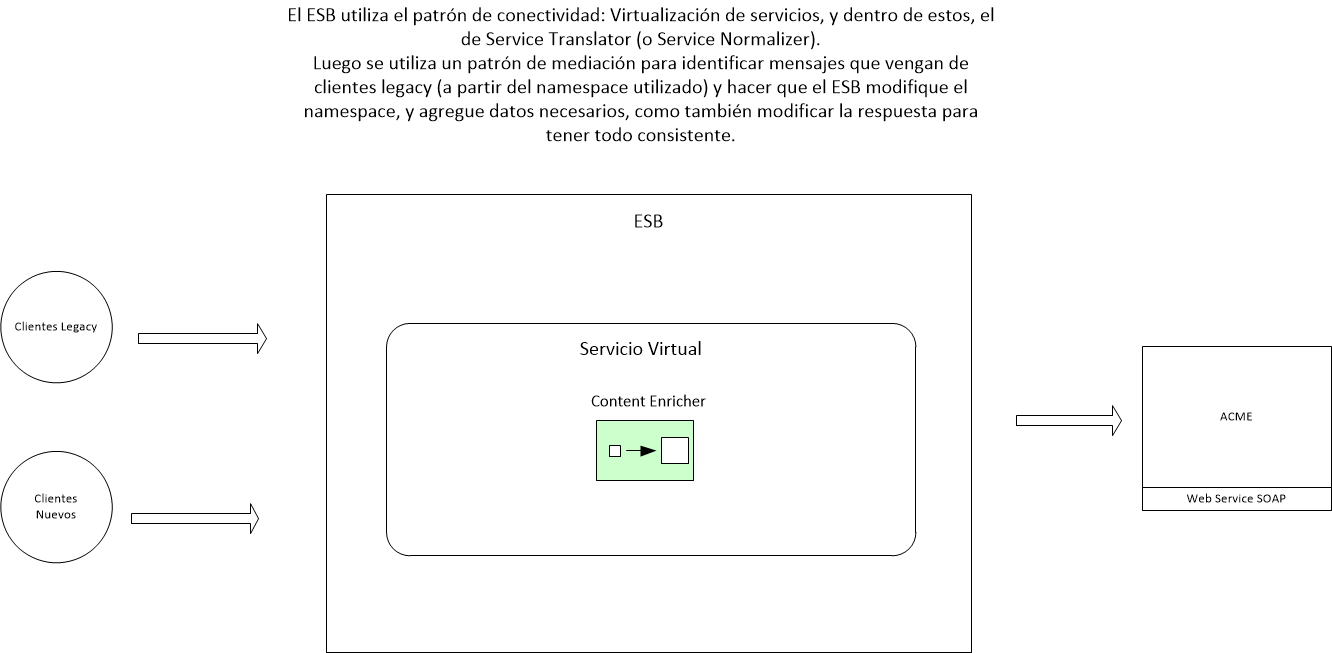
\includegraphics[scale=0.5]{../acmeesb/arq.png}
  \caption{Arquitectura Sistema}
  \label{fig:arq}
\end{figure} 


Básicamente en la figura \ref{fig:diagrama} se presenta la implementación del Middleware, para la realización del mismo se utilizó Mule ESB, un framework completo para la implementación de conectores, componentes y funcionalidades adicionales, que permiten en alto nivel definir la lógica de negocio en forma precisa y sencilla.

\begin{landscape}
  \begin{figure}[!h]
  \centering
    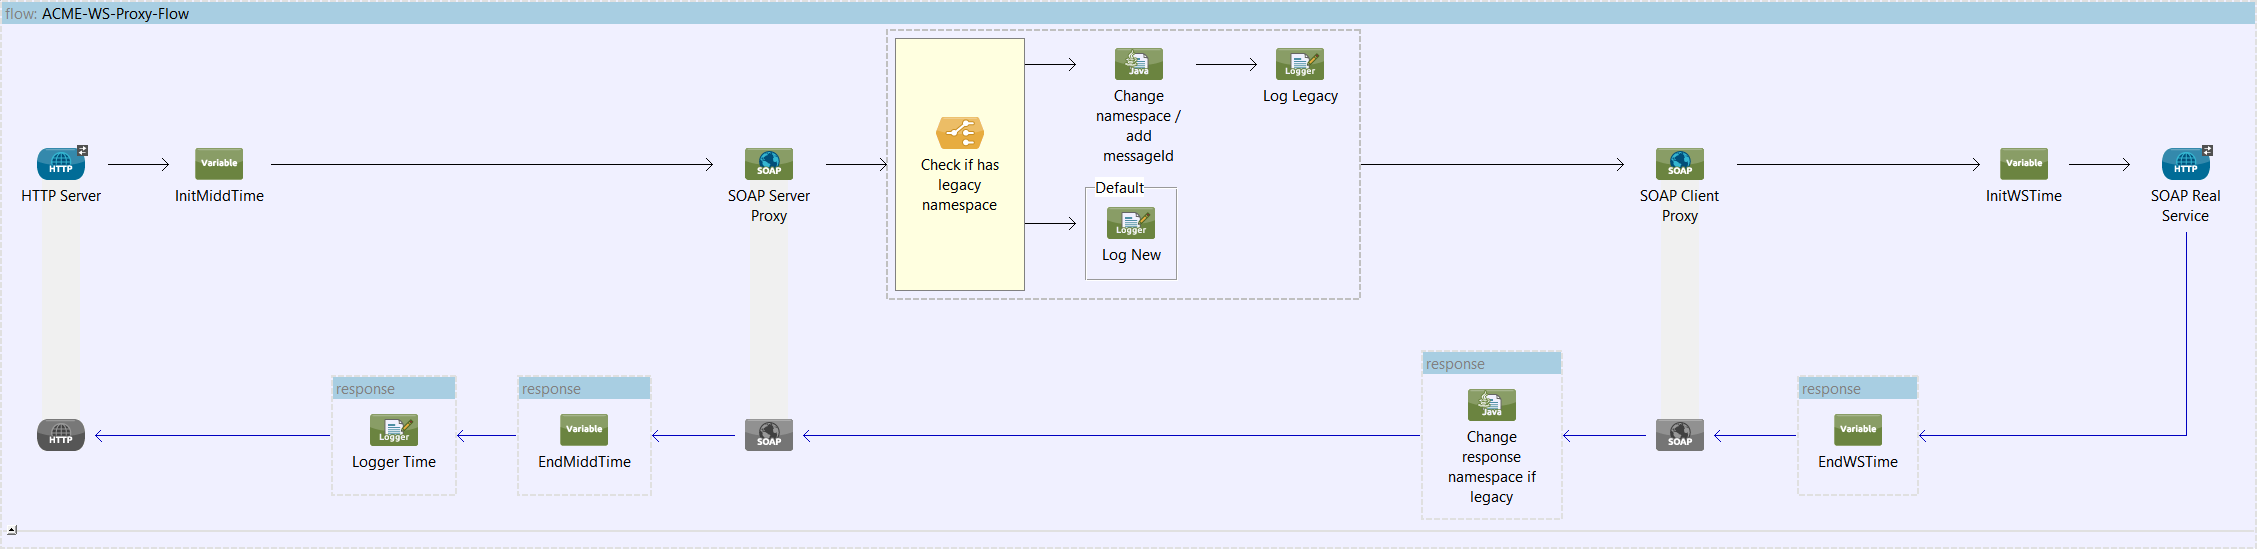
\includegraphics[scale=0.27]{../acmeesb/ACME-WS-Proxy-Flow.png}
  \caption{Arquitectura Middleware}
  \label{fig:diagrama}
\end{figure} 
\end{landscape}


Lo que respecta la implementación se procederá a la explicación por componente, siguiendo el flujo de la lógica de negocio. Se separará en subesquemas para mejor comprensión del flujo.
Para la figura \ref{fig:g1} incluímos un HTTP Endpoint[1] para recibir las solicitudes vía HTTP, para ello utilizamos un patrón request-response debido a que el servicio web implementado tiene una respuesta al cliente. Para el conector utilizamos el puerto 8081.
El item InitMiddTime es un Transformer del tipo variable, el cual es utilizado para la métrica de calidad del tiempo de respuesta del Middleware, la idea básica consiste en instanciar una variable llamada $initM$ llamando a la función $server.nanoTime()$ devolviendo el tiempo en nanosegundos.
El ítem SOAP Service Proxy consiste en un componente del tipo CXF publicando un proxy SOAP utilizando JAX-WS. La 
idea principal de este componente es brindar la capacidad de recibir solicitudes de servicios con distintas versiones, por lo tanto la operación para el mismo es de $Proxy Service$, el cual dado una solicitud HTTP devuelve en el payload un XML(envelope) el cual será procesado en el siguiente subesquema del flujo. El servicio se llama $transactions$ y el namespace del mismo es $ACMEv1$.

  \begin{figure}[!h]
  \centering
    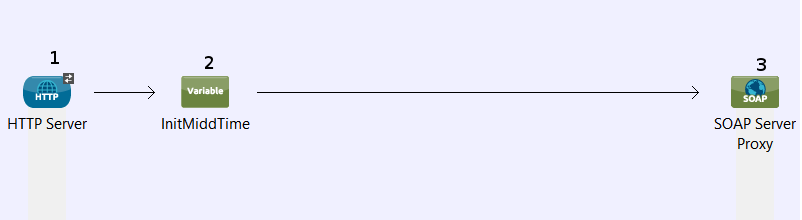
\includegraphics[scale=0.5]{./images/g1.png}
  \caption{HTTP endpoint - Variable - CXF}
  \label{fig:g1}
\end{figure} 

Una vez generado el proxy a través de los conectores apropiados, se procede a la tarea de procesar los pedidos, es decir, se modificará de forma adecuada las solicitudes de forma tal que cumpla con los requerimientos y formatos propuestos por el Webservice de la versión nueva(ACMEv1), esto implica a grandes rasgos, detectar el namespace de la solicitudes, en caso de que el namespace del XML en cuestión sea una versión antigua del servicio(ACME), se procede a introducir el nuevo atributo para identificar los grupos el mismo se llama $messageId$.
En la figura \ref{fig:g2} se destaca el Flow Control Choice llamado $Check$ $if$ $has$ $legacy$ $namespace$, el cual evalúa mediante una expresión adecuada y selecciona el flujo correcto por el cual continuará el proceso.
Básicamente mediante la expresión $xpath://*[namespace-uri()='ACME']$ filtra adecuadamente el flujo. Es decir, si el namespace root corresponde a una versión antigua del servicio se seleccionará el flujo que tiene un componente Java, caso contrario se procederá al registro en un log del sistema. \\

El componente Java se encarga de dos funcionalidades principales:
\begin{enumerate}
  \item Cambiar el namespace "ACME" por "ACMEv1".
  \item Agregar el elemento $messageId$ al payload.
\end{enumerate}
Se trata de una clase Java llamada $TransformXML$ que implementa la clase $Callable$ brindada por la API de Mule. Para ello se sobrescribe la función $onCall$ con parámetro de entrada $MuleEventContext$, el cual posee el mensaje y demás parámetros relativos al contexto de la aplicación. Se utiliza la clase $dom4j$ para transformar el payload del mensaje en un documento de esa clase, posteriormente agregar el nodo adecuado dentro de la estructura XML.
Para generar el valor del nodo $messageId$ se toma como referencia el XML como String, y se genera utilizando un algoritmo $SHA-256$ de 16 caracteres para obtener un identificador unívoco y de esta forma evitar transacciones de la misma solicitud. El valor final entonces para $messageId$ será $legacy-sha256(XML)$. Una vez finalizado los dos procesos principales, se procede a agregar una variable de sesión con nombre $isLegacy$, la cual será utilizada como referencia para codificar la respuesta del servicio en caso que el namespace filtrado sea "ACME". Finalmente se devuelve el payload del mensaje, es decir un $Document$ provisto por el paquete $dom4j$ que representa el XML para posterior procesamiento.

Posterior a la salida del componente Java, se registra en log a nivel de información, indicando que el mensaje es de un cliente legacy y se le ha agregado $messageId$. Este log se nombra "Log Legacy".
Para el segundo flujo en el cual el mensaje pertenece a un cliente nuevo, únicamente se procederá al log a nivel de información destacando que la solicitud pertenece a un cliente que utiliza la versión cuyo namespace es "ACMEv1".
El payload del mensaje al finalizar el flujo es un Document perteneciente al paquete $dom4j$ que representa el XML, el cual será directamente redirigido hacia el servicio web en su reciente versión, con el namespace correctamente ajustado y los atributos agregados en caso de tratarse de solicitudes legacy.

  \begin{figure}[!h]
  \centering
    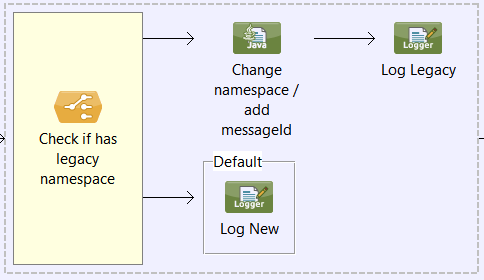
\includegraphics[scale=0.7]{./images/g2.png}
  \caption{Lógica}
  \label{fig:g2}
\end{figure} 

El subesquema \ref{fig:g3} es análogo a \ref{fig:g1}, pero en este caso se realiza la invocación al servicio web, y se ajusta una nueva variable en el componente $InitWSTime$ que se utiliza como referencia para medir el tiempo de de respuesta del servicio web.

  \begin{figure}[!h]
  \centering
    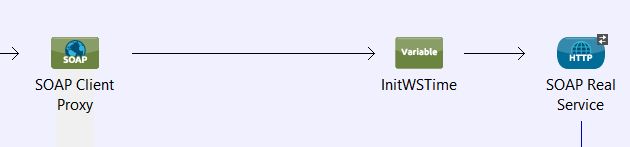
\includegraphics[scale=0.6]{./images/g3.png}
  \caption{CXF - Variable - HTTP endpoint}
  \label{fig:g3}
\end{figure} 

Una vez realizada la operación del servicio web, el Middleware obtiene como respuesta que debe ser reenviada nuevamente a los clientes que solicitaron el pedido. En el subesquema \ref{fig:g4} consta de un Transformer de tipo Variable, el cual inicializa una variable con el nombre $endWS$ y valor llamando la función $server.nanoTime()$, para obtener el tiempo final de ejecución del servicio web.
El componente Java con nombre $Change$ $response$ $namespace$ $if$ $legacy$ como lo dice el mismo, cambia el namespace de la respuesta del servicio web por el correspondiente, para eso obtiene la variable de sesión $isLegacy$ ajustada en el componente Java anteriormente descripto y ajusta el namespace "ACME", si dicha variable posee como valor $true$. Caso contrario el payload del mensaje no sufre cambios y se realiza el fordwarding correspondiente.
El componente Java se invoca utilizado la clase $org.midd.customtransformer.ParserComponent$ que implementa nuevamente $Callable$. Como proceso final se devuelve en el payload del mensaje un objeto del tipo $Document$ provisto en el paquete $dom4j$.

\begin{figure}[!h]
  \centering
    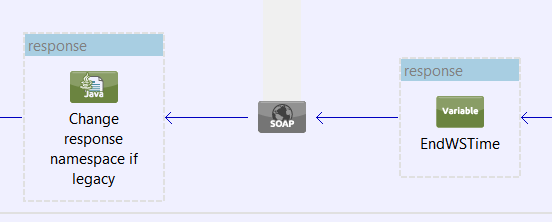
\includegraphics[scale=0.7]{./images/g4.png}
  \caption{CXF - Variable - HTTP endpoint}
  \label{fig:g4}
\end{figure} 


Por lo tanto, se debe tener en cuenta los namespaces en ambos sentidos send-receive, ya que al tratarse de clientes legados, se debe transformar los mensajes tanto de request como de reply. El mecanismo parece ser solvente y definitivamente cumple con uno de los objetivos del sistema Middleware, permitir la interacción entre sistemas legados e implementaciones del servicio actuales. Sin dudas se puede considerar como una buena solución la inclusión de un sistema Middleware cuando se trata de unificar servicios web, aunque lo ideal sería la inclusión de dicho sistema en diversos puntos, de esta forma se logra balancear la carga de request de los clientes, no saturando el servicio nuevo implementado.

\subsection{Versionado WS}
En esta sección se describe la estrategia utilizada para el versionado del web service dado el contexto de los requerimientos de la aplicación.
Se optó por la estrategia FLEXIBLE debido a que se pueden generar cambios del tipo compatibles hacia atrás, de esta forma utilizamos la notación $X.YY$, en la cual $X$ indica una versión mayor, en este caso se introducen cambios en el contrato que son incompatibles, mientras que $YY$ denota versiones menores, realizando cambios compatibles hacia atrás, como por ejemplo agregar un nuevo atributo opcional. Entonces se obtienen los siguientes detalles del sistema de versionado:
\begin{itemize}
  \item Cambios versiones mayores($X$): Cuando se agrega un cambio en el contrato donde no exista compatibilidad hacia atrás, se incrementa la versión mayor una unidad, y la versión menor $YY$ se le asigna $0$, de esta forma tendremos diversos conjuntos de clientes legados y clientes compatibles en una versión dada.
  \item Cambios versiones menores($YY$): En este caso se realizan cambios en el contrato que permiten compatibilidad entre las versiones. Por ejemplo se añade un atributo opcional en el esquema.
\end{itemize}
Existe una serie de problemáticas relativas a la implementación de los web services. Como primeramente se genera el código y posteriormente el servicio, esto implica la generación del WSDL, XSD y WS-Policy, no se tiene control absoluto sobre las versiones, puesto que los XSD se generan de forma automática, heredando de esta forma el targetnamespace del WSDL. Dadas las limitaciones a nivel de implementación, no se realizará versionado de los XSD, los mismos heredarán el targetnamespace del WSDL.

\subsubsection{Cambios}
La versión mayor se referenciará en el targetnamespace del WSDL, de esta forma genera errores en los clientes legados que invoquen un servicio con una versión incompatible. De esta forma el targetnamespace será de la forma $ACMEvX$ donde $X$ corresponde a la versión mayor. Recordemos que la versión anterior implementada poseía un targetnamespace $ACME$. Entonces el primer cambio realizado es el targetnamespace de $ACME$ a $ACMEv1$.
La nomenclatura completa se referencia en una etiqueta del WSDL de la forma $<wsdl:documentation>Version: X.YY</wsdl:documentation>$.
Los cambios a nivel de implementación fueron los siguientes:
\begin{itemize}
  \item Migración de servidor web Apache Tomcat a JBoss Application Server 7, de esta forma poder utilizar apache CXF como ser el caso de $documentation$ para indicar la versión completa del WSDL.
  \item Agregar targetnamespace al WebService, en este caso con el modelo de versionado propuesto. Esto se logra agregando el annotation $@WebService$ e incluyendo como targetnamesace $ACMEv1$ en la clase TransactionsWS.java.
  \item De forma análoga se logra incluir el tag de documentation en el WSDL, esto se lleva a cabo agregando la annotation $@WSDLDocumentation$ incluyendo el valor de la versión, así como la ubicación del tag en el WSDL.
\end{itemize}


Para el targetnamespace, se debe proceder a definir lo siguiente antes de definir la clase del web service:
\begin{center}
    @WebService(name = "transactions", serviceName = "transactions", 
                portName="transactionsPort", targetNamespace="ACMEv1");
\end{center}

De forma análoga se procede para el tag de versionado incluyendo la siguiente linea antes de definir la clase:
\begin{center}
  @WSDLDocumentation(value = "Version: 1.0", placement = WSDLDocumentation.Placement.TOP)
\end{center}

\section{Modelo de Calidad}
En la actualidad existe en la industria un creciente interés por la especificación de los aspectos no funcionales, o de calidad, de los servicios. Para cumplir con estas necesidades es que aparecen los Modelos de Calidad que generalmente se centran en la identificación y clasificación de distintos factores de calidad que se organizan en forma jerárquica y se documentan en dichos modelos.
Para el presente laboratorio utilizaremos un Modelo de Calidad basado en el S-Cube estudiado en el teórico, haciendo foco en la dimensión la “Performance” y utilizando como factor o atributo de calidad el “tiempo de respuesta”. Cabe destacar que el tiempo de respuesta en  S-Cube es solo uno de los atributos de calidad asociados a la Performance, por lo tanto para tener una visión más precisa de la calidad del web service en lo relacionado a la Performance se deberían aplicar métodos para obtener las métricas de los restantes atributos (Tiempo de transacción, throughput, latencia, tiempo de ejecución, latencia de cola), sin embargo el tiempo de respuesta es el único que se pide para el presente obligatorio.
La métrica utilizada como instrumento de medida para el factor “tiempo de respuesta” es la siguiente. Se medirá a partir de la implementación de timestamps a nivel de ESB, que miden los tiempos desde que un mensaje llega al middleware hasta que sale del mismo (con exactitud de nanosegundos), obteniendo mediciones intermedias correspondientes al tiempo de procesamiento solo de la llamada al web service en el back end.
Para realizar las pruebas finalmente se utilizó la herramienta SOAPUI para enviar un conjunto de datos simple y reducido (3 transacciones validas) al ESB de forma secuencial uno por uno.
Los resultados de las pruebas tanto para el cliente Legacy como el Nuevo, se encuentran en las tablas tabla[\ref{tabla:datoslegacy}] y tabla[\ref{tabla:datosnew}] respectivamente.

\begin{table}
\begin{center}
    \begin{tabular}{| c | c | c | c |}
\hline
    \multicolumn{1}{|c}{Caso}&
    \multicolumn{1}{|c}{RespMidd}&
    \multicolumn{1}{|c|}{RespWS}&
    \multicolumn{1}{|c|}{RespOnlyMidd} \\ \hline
    
1 & 19.350741 & 5.301935 &14.048806\\ \hline
2 & 17.05937 & 3.929897 & 13.129473\\ \hline
3 & 15.619519 & 4.548652 & 11.070867\\ \hline
4 & 15.439171 &4.617932 &10.821239\\ \hline
5 & 17.269775 & 4.503932 & 12.765843\\ \hline
6 & 20.231219 & 6.407482 & 13.823737\\ \hline
7 & 15.416077 & 4.201519 & 11.214558\\ \hline
8 & 16.168993 & 4.933174 & 11.235819\\ \hline
9 & 16.717368 & 4.724602 & 11.992766\\ \hline
10 & 16.568911 & 4.771887 & 11.797024\\ \hline
Prom & 16.9841144 & 4.7941012 & 12.1900132 \\ \hline%%prom

    \end{tabular}
\end{center}
    \caption{Métricas Legacy}
    \label{tabla:datoslegacy}
\end{table}



\begin{table}
\begin{center}
    \begin{tabular}{| c | c | c | c |}
\hline
    \multicolumn{1}{|c}{Caso}&
    \multicolumn{1}{|c}{RespMidd}&
    \multicolumn{1}{|c|}{RespWS}&
    \multicolumn{1}{|c|}{RespOnlyMidd} \\ \hline
    
1 & 9.019593 & 4.809227 &4.210316\\ \hline
2 & 6.933862 & 4.084953 &2.848909\\ \hline
3 & 7.444848 & 4.058927 &3.385921\\ \hline
4 & 7.717569 & 4.033268 &3.684301\\ \hline
5 & 7.138771 & 3.877846 &3.260925\\ \hline
6 & 6.84992 & 3.850354 & 2.999566\\ \hline
7 & 7.41589 & 4.215082 & 3.200808\\ \hline
8 & 9.496855 & 5.823917 & 6.672938\\ \hline
9 & 7.883621 & 4.851065 & 3.032556\\ \hline
10 & 7.483704 & 4.351442 & 3.132262\\ \hline
Prom & 7.7384633 & 4.3956081 & 3.6428502\\ \hline

    \end{tabular}
\end{center}
    \caption{Métricas Nuevo}
    \label{tabla:datosnew}
\end{table}


RespMidd: Es el tiempo del mensaje en el middleware ignorando el tiempo de red entre el cliente y el ESB (todas las mediciones se realizan dentro del mismo). Además no se tiene en cuenta el tiempo de parseo del pedido HTTP a mensaje ESB y viceversa pero son considerados despreciables.
RespWS: Tiempo desde que el ESB envía el pedido al WS hasta que recibe la respuesta
RespOnlyMidd: Es RespMidd-RespWS, dando como resultado solo el tiempo de procesamiento del ESB.
Analizando los resultados y observando los promedios en cada caso podemos sacar como conclusiones que:
\begin{itemize}
  \item El tiempo de respuesta del WS permanece incambiado para los casos de clientes Legacy y Nuevos, encontrándose en el entorno de los 4.5ms.
  \item El tiempo de procesamiento dentro del middleware para el caso de los clientes Legacy es mucho mayor debido a los procesamientos para que se adapte a consumir el nuevo servicio, encontrándose en el entorno de los 12ms contra los 3.5ms para el caso de los clientes nuevos.
\end{itemize}

Estos resultados si bien fueron medidos en un entorno de desarrollo ( por lo que los resultados podrían ser ligeramente diferentes en producción), son considerados representativos para medir la performance del sistema en condiciones normales.


%\bibliographystyle{abbrv}
%\bibliography{simple}

\end{document}
